\section{Euler's method} \label{S:7.3.Euler}

\vspace*{-14 pt}
\framebox{\hspace*{3 pt}
\parbox{\boxwidth}{\begin{goals}
\item What is Euler's method and how can we use it to approximate the
  solution to an initial value problem?  
\item How accurate is Euler's method?
\end{goals}} \hspace*{3 pt}}

\subsection*{Introduction}

In Section~\ref{S:7.2.Qualitative}, we saw how a slope field can be used to sketch
solutions to a differential equation.  In particular, the slope field
is a plot of a large collection of tangent lines to a large number of solutions of the
differential equation, and we sketch a single solution by simply following
these tangent lines.  With a little more thought, we may use this same
idea to numerically approximate the solutions of a differential equation.  

\begin{pa} \label{PA:7.3}
Consider the initial value problem 
$$
\frac{dy}{dt} = \frac12 (y + 1), \ y(0) = 0.
$$
\ba
\item Use the differential equation to find the slope of the tangent
  line to the solution $y(t)$ at $t=0$.  Then use the given initial value to
  find the equation of the tangent line at $t=0$.  

\item Sketch the tangent line on the axes below on the interval $0\leq
  t\leq 2$ and use it to approximate $y(2)$,
  the value of the solution at $t=2$.   

  \begin{center}
    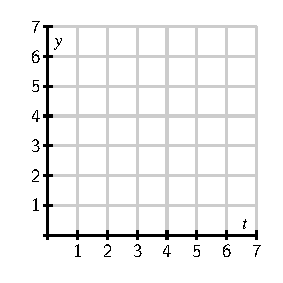
\includegraphics{figures/7_3_PA.eps}
  \end{center}

\item Assuming that your approximation for $y(2)$ is the actual value
  of $y(2)$, use the differential equation to find the slope of the
  tangent line to $y(t)$ at $t=2$.  Then, write the equation of the
  tangent line at $t=2$.  

\item Add a sketch of this tangent line to your plot on the axes above on the interval $2\leq
  t\leq 4$; use this new tangent line to approximate $y(4)$,
  the value of the solution at $t=4$.   

\item Repeat the same step to find an approximation for $y(6)$.

\ea
\end{pa} 
\afterpa


\subsection*{Euler's Method} \index{Euler's Method}

Preview Activity~\ref{PA:7.3} demonstrates the essence of an algorithm, which is known as
Euler's Method, that generates a numerical approximation to the solution
of an initial value problem.\footnote{``Euler'' is pronounced
  ``Oy-ler.''  Among other things, Euler is the mathematician credited with the famous number $e$; if you incorrectly pronounce his name ``You-ler,'' you fail to appreciate his genius and legacy.}  In this algorithm, we
will approximate the solution by taking horizontal steps of a fixed
size that we denote by $\Delta t$.  

Before explaining the algorithm in detail, let's remember how we
compute the slope of a line:  the slope is the ratio of the vertical
change to the horizontal change, as shown in the following figure.

\begin{center}
  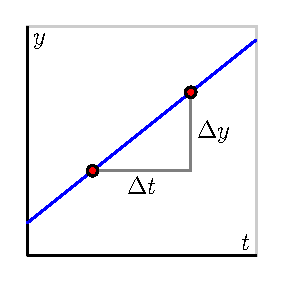
\includegraphics{figures/7_3_slope.eps}
\end{center}
In other words, $m = \frac{\Delta y}{\Delta t}$.  Said differently, the
vertical change is the product of the slope and the horizontal change:
$$\Delta y = m\Delta t.$$

Suppose that we would like to solve the initial value problem
$$
  \frac{dy}{dt} = t - y, \ y(0) = 1.
$$
While there is an algorithm by which we can find an algebraic formula for the solution to this initial value problem, and we can check that this solution is $y(t) = t -1 + 2e^{-t}$, we are instead interested in generating an approximate solution by creating a sequence
of points $(t_i, y_i)$, where $y_i\approx y(t_i)$.  For this first example, we choose $\Delta t = 0.2$.

\medskip

\noindent \begin{minipage}[l]{3.6in}
Since we know that $y(0) = 1$, we will take the initial point to be
$(t_0,y_0) = (0,1)$ and move horizontally by $\Delta t = 0.2$ to the
point $(t_1,y_1)$.  Therefore, $t_1=t_0+\Delta t = 0.2$. 
The differential equation tells us that the slope of the 
tangent line at this point is
$$
m=\frac{dy}{dt}\bigg\vert_{(0,1)} = 0-1 = -1.
$$
Therefore, if we move along the tangent line by taking a horizontal
step of size $\Delta t=0.2$, we must also move vertically by
$$\Delta y = m\Delta t = -1\cdot 0.2 = -0.2.$$  We then have the
approximation $y(0.1) \approx y_1= y_0 + \Delta y = 1 - 0.2 = 0.8.$  At this point, we have executed one step of Euler's method.
\end{minipage}
\hspace*{.25in}
\begin{minipage}[l]{2in}
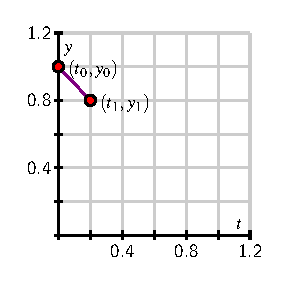
\includegraphics{figures/7_3_euler_points_1.eps}
\end{minipage}

\medskip
\noindent \begin{minipage}[l]{3.6in}
Now we repeat this process:  at $(t_1,y_1) = (0.2,0.8)$, the
differential equation tells us that the slope is 
$$
m=\frac{dy}{dt}\bigg\vert_{(0.2,0.8)} = 0.2-0.8 = -0.6.
$$
If we move horizontally by $\Delta t$ to $t_2=t_1+\Delta = 0.4$, we must move
vertically by
$$
\Delta y = -0.6\cdot0.2 = -0.12.
$$
We consequently arrive at $y_2=y_1+\Delta y = 0.8-0.12 = 0.68$, which
gives $y(0.2)\approx 0.68$.  Now we have completed the second step of Euler's method.


\end{minipage}
\hspace*{0.25in}
\begin{minipage}[c]{2in}
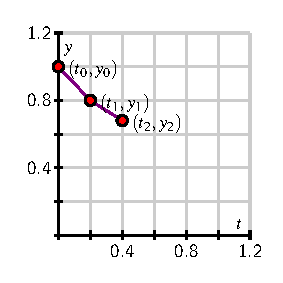
\includegraphics{figures/7_3_euler_points_2.eps}
\end{minipage}

\medskip

If we continue in this way, we may generate the points $(t_i, y_i)$
shown at left in Figure~\ref{F:7.3.EulerPts}.  In situations where we are able to find a formula for the actual solution $y(t)$, we can graph $y(t)$ to compare it to the points generated by Euler's method, as shown at right in Figure~\ref{F:7.3.EulerPts}.
\begin{figure}[h]
\begin{center}
\scalebox{0.9}{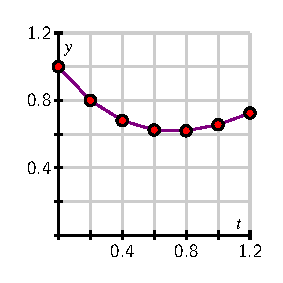
\includegraphics{figures/7_3_euler_points_6.eps}}  \hspace{0.25in}
  \scalebox{0.9}{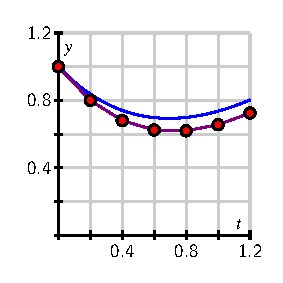
\includegraphics{figures/7_3_euler.eps}}
\end{center}
\caption{At left, the points and piecewise linear approximate solution generated by Euler's method; at right, the approximate solution compared to the exact solution (shown in blue).} \label{F:7.3.EulerPts}
\end{figure}


Because we need to generate a large number of points $(t_i,y_i)$, it is convenient to organize the implementation of Euler's method in a
table as shown.  We begin with the given initial data.

\begin{center}
\begin{tabular}{|c|c|c|c|c|}
  \hline
  $t_i$&$y_i$&$dy/dt$&$\Delta y$\\
  \hline
  0.0000&1.0000&\hphantom{-1.0000} & \hphantom{-0.2000}\\
  \hline
\end{tabular}
\end{center}
\noindent
From here, we compute the slope of the tangent line $m=dy/dt$ using
the formula for $dy/dt$ from the differential 
equation, and then we find $\Delta y$, the change in $y$, using the rule $\Delta y = m\Delta t$.

\begin{center}
\begin{tabular}{|c|c|c|c|c|}
  \hline
  $t_i$&$y_i$&$dy/dt$&$\Delta y$\\
  \hline
  0.0000&1.0000&-1.0000&-0.2000\\
  \hline
\end{tabular}
\end{center}
\noindent
Next, we increase $t_i$ by $\Delta t$ and $y_i$ by $\Delta y$ to get
\noindent
\medskip
\begin{center}
\begin{tabular}{|c|c|c|c|c|}
  \hline
  $t_i$&$y_i$&$dy/dt$&$\Delta y$\\
  \hline
  0.0000&1.0000&-1.0000&-0.2000\\ \hline
  0.2000&0.8000& & \\
  \hline
\end{tabular}
\end{center}
\noindent
and then we simply continue the process for however many steps we decide, eventually generating a table like the one that follows.
\medskip
\begin{center}
\begin{tabular}{|c|c|c|c|c|}
  \hline
  $t_i$&$y_i$&$dy/dt$&$\Delta y$\\
  \hline
  0.0000&1.0000&-1.0000&-0.2000\\ \hline
  0.2000&0.8000&-0.6000&-0.1200\\ \hline
  0.4000&0.6800&-0.2800&-0.0560\\ \hline
  0.6000&0.6240&-0.0240&-0.0048\\ \hline
  0.8000&0.6192&0.1808&0.0362\\ \hline
  1.0000&0.6554&0.3446&0.0689\\ \hline
  1.2000&0.7243&0.4757&0.0951\\ 
  \hline
\end{tabular}
\end{center}



\begin{activity} \label{A:7.3.1}  
Consider the initial value problem
$$
  \frac{dy}{dt} = 2t-1, \ y(0) = 0
  $$
\ba

	\item Use Euler's method with $\Delta t = 0.2$ to approximate the solution
at $t_i = 0.2, 0.4, 0.6, 0.8$, and $1.0$.   Record your work in the following table, and sketch the points $(t_i,
y_i)$ on the following axes provided.

  \begin{tabular}{|c|c|c|c|c|}
  \hline
  \vphantom{\Huge{M}}$t_i$&$y_i$&$dy/dt$&$\Delta y$\\
  \hline
  \hline
  \vphantom{\Huge{M}}0.0000&0.0000&\hphantom{1.0000}&\hphantom{0.2000} \\
  \hline
  \vphantom{\Huge{M}}0.2000&\hphantom{MMMMMM} 
  & \hphantom{MMMMMM} & \hphantom{MMMMMM} \\
  \hline
  \vphantom{\Huge{M}}0.4000& & & \\
  \hline
  \vphantom{\Huge{M}}0.6000& & & \\
  \hline
  \vphantom{\Huge{M}}0.8000& & & \\
  \hline
  \vphantom{\Huge{M}}1.0000& & & \\
  \hline
\end{tabular}

\scalebox{1.15}{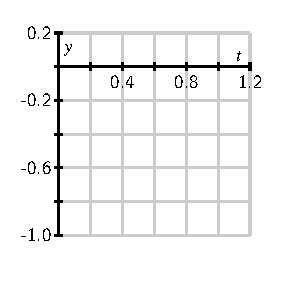
\includegraphics{figures/7_3_euler_empty.eps}}

\item Find the exact solution to the original initial value problem
  and use this function to find the error in your approximation at each one of the points
  $t_i$.

\item Explain why the value $y_5$ generated by Euler's method for this initial value problem
  produces the same value as a left Riemann sum for the definite integral $\int_0^1
  (2t-1)~dt$.  

\item How would your computations differ if the initial value was $y(0) =
  1$?  What does this mean about different solutions to this
  differential equation?   

\ea
\end{activity}
\begin{smallhint}
\ba
	\item Small hints for each of the prompts above.
\ea
\end{smallhint}
\begin{bighint}
\ba
	\item Big hints for each of the prompts above.
\ea
\end{bighint}
\begin{activitySolution}
\ba
	\item Solutions for each of the prompts above.
\ea
\end{activitySolution}
\aftera

\newpage

\begin{activity} \label{A:7.3.2}  
Consider the differential equation
$
  \frac{dy}{dt} = 6y-y^2
$.
\ba
\item Sketch the slope field for this differential equation on the axes provided at left below.

\begin{center}
  \scalebox{1.1}{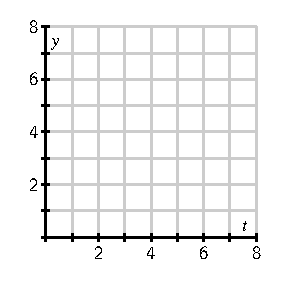
\includegraphics{figures/7_3_slopefield.eps}} \hspace{0.2in}  \scalebox{1.1}{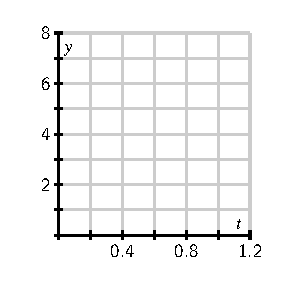
\includegraphics{figures/7_3_euler_empty_2.eps}}
\end{center}

\item Identify any equilibrium solutions and determine whether they
  are stable or unstable.   

\item What is the long-term behavior of the solution that satisfies the initial
  value $y(0) = 1$?

\item Using the initial value $y(0) = 1$, use Euler's method with
  $\Delta t = 0.2$ to approximate the solution at $t_i = 0.2, 0.4,
  0.6, 0.8$, and $1.0$.  Sketch the points $(t_i, y_i)$ on the axes provided at right in (a).  (Note the different horizontal scale on the two sets of axes.)

  \begin{tabular}{|c|c|c|c|c|}
  \hline
  $t_i$&$y_i$&$dy/dt$&$\Delta y$\\
  \hline
  \hline
  \vphantom{\Huge{M}}0.0&1.0000&\hphantom{1.0000}&\hphantom{0.2000} \\
  \hline
  \vphantom{\Huge{M}}0.2&\hphantom{MMMMMM} 
  & \hphantom{MMMMMM} & \hphantom{MMMMMM} \\
  \hline
  \vphantom{\Huge{M}}0.4& & & \\
  \hline
  \vphantom{\Huge{M}}0.6& & & \\
  \hline
  \vphantom{\Huge{M}}0.8& & & \\
  \hline
  \vphantom{\Huge{M}}1.0& & & \\
  \hline
\end{tabular}



\item What happens if we apply Euler's method to approximate the
  solution with $y(0) = 6$?

\ea
\end{activity}
\begin{smallhint}
\ba
	\item Small hints for each of the prompts above.
\ea
\end{smallhint}
\begin{bighint}
\ba
	\item Big hints for each of the prompts above.
\ea
\end{bighint}
\begin{activitySolution}
\ba
	\item Solutions for each of the prompts above.
\ea
\end{activitySolution}
\aftera

\subsection*{The error in Euler's method} \index{Euler's Method!error}

Since we are approximating the solutions to an initial value problem
using tangent lines, we should expect that the error in the
approximation will be less when the step size is smaller.
To explore this observation quantitatively, let's consider the initial value problem
$$
  \frac{dy}{dt} = y, \ y(0) = 1
$$
whose solution we can easily find.

Consider the question posed by this initial value problem: ``what function do we know that is the same as its own
derivative and has value 1 when $t=0$?'' It is not hard to see that the 
solution is $y(t) = e^t$.    We now apply Euler's method
to approximate $y(1) = e$ using several values of $\Delta t$.  These
approximations will be denoted by $E_{\Delta t}$, and these estimates provide us a way to see how accurate Euler's Method is.

To begin, we apply Euler's method with a step size of $\Delta t =
0.2$.  In that case, we find that $y(1) \approx E_{0.2} = 2.4883$.  The
error is therefore $y(1) - E_{0.2} = e - 2.4883 \approx 0.2300$.

Repeatedly halving $\Delta t$ gives the following
results, expressed in both tabular and graphical form.

\begin{center}
\begin{minipage}[c]{2.0in}
\begin{tabular}{|c|c|c|}
  \hline
  $\Delta t$ & $E_{\Delta t}$ & Error \\
  \hline
  0.200&2.4883&0.2300\\
  0.100&2.5937&0.1245\\
  0.050&2.6533&0.0650\\
  0.025&2.6851&0.0332\\
  \hline
\end{tabular}
\end{minipage}
\hspace*{0.25in}
\begin{minipage}[c]{2.0in}
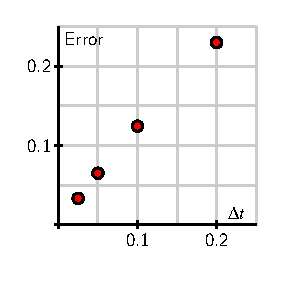
\includegraphics{figures/7_3_error.eps}
\end{minipage}
\end{center}

Notice, both numerically and graphically, that the error is roughly halved when $\Delta t$ is halved.
This example illustrates the following general principle.

\vspace*{5pt}
\nin \framebox{\hspace*{3 pt}
\parbox{\boxwidth}{
    If Euler's method is to approximate the solution to an initial
    value problem at a point $\overline{t}$, then the error is
    proportional to $\Delta t$.  That is,
    $$
    y(\overline{t}) - E_{\Delta t} \approx K\Delta t
    $$
    for some constant of proportionality $K$.

} \hspace*{3 pt}}
\vspace*{1pt}

\newpage

\begin{summary}
\item Euler's method is an algorithm for approximating the solution to
  an initial value problem by following the tangent lines while we
  take horizontal steps across the $t$-axis.
\item If we wish to approximate $y(\overline{t})$ for some fixed
  $\overline{t}$ by taking horizontal steps of size $\Delta t$, then the
  error in our approximation is proportional to $\Delta t$.  
\end{summary}

\nin \hrulefill

\begin{exercises} 
  \item  Newton's Law of Cooling says that the rate at which an
    object, such as a cup of coffee, cools is proportional to the
    difference in the object's temperature and room temperature.  If
    $T(t)$ is the object's temperature and $T_r$ is room temperature,
    this law is expressed at
    $$
    \frac{dT}{dt} = -k(T-T_r),
    $$
    where $k$ is a constant of proportionality.  In this problem,
    temperature is 
    measured in degrees Fahrenheit and time in minutes.

    \ba
    \item  Two calculus students, Alice and Bob, enter a 70$^\circ$
    classroom at the same time.  Each has a cup of coffee that is
    100$^\circ$.  The differential equation for Alice has a constant
    of proportionality $k=0.5$, while the constant of proportionality
    for Bob is $k=0.1$.

    What is the initial rate of change for Alice's coffee? 
    What is the initial rate of change for Bob's coffee?

    \item  What feature of Alice's and Bob's cups of coffee could explain
    this difference?

 \item  As the heating unit turns on and off in the room, the
    temperature in the room is $$T_r=70+10\sin t.$$  Implement Euler's
    method with a step size of $\Delta t = 0.1$ to approximate the
    temperature of Alice's coffee over the time interval $0\leq t\leq
    50$.  This will most easily be performed using a spreadsheet such
    as \emph{Excel}.  Graph the temperature of her coffee and room
    temperature over this interval.

   \item  In the same way, implement Euler's method to approximate the
    temperature of Bob's
    coffee over the same time interval.  Graph the temperature of his
    coffee and room temperature over the interval.

    \item  Explain the similarities and differences that you see in the
    behavior of Alice's and Bob's cups of coffee.
\ea

  \item We have seen that the error in approximating the solution to
    an initial value problem is proportional to $\Delta t$.  That is,
    if $E_{\Delta t}$ is the Euler's method approximation to the
    solution to an initial value problem at $\overline{t}$, then
    $$y(\overline{t})-E_{\Delta t} \approx K\Delta t
    $$
    for some constant of proportionality $K$.

    In this problem, we will see how to use this fact to improve our
    estimates, using an idea called {\em accelerated convergence}.

    \ba
    \item  We will create a new approximation by assuming the error is
    {\em exactly} proportional to $\Delta t$, according to the formula
    $$y(\overline{t})-E_{\Delta t} =K\Delta t.
    $$
    
    Using our earlier results from the initial value problem $dy/dt = y$ and
    $y(0)=1$ with $\Delta t = 0.2$ and $\Delta t = 0.1$, we have
    \begin{eqnarray*}
      y(1) - 2.4883 & = & 0.2K \\
      y(1) - 2.5937 & = & 0.1K. \\
    \end{eqnarray*}

    This is a system of two linear equations in the unknowns $y(1)$
    and $K$.  Solve this system to find a new approximation for
    $y(1)$.  (You may remember that the exact value is $y(1) = e =
    2.71828\ldots.$)

    \item Use the other data, $E_{0.05} = 2.6533$ and $E_{0.025} = 2.6851$
    to do similar work as in (a) to obtain another approximation.  Which gives the better
    approximation?  Why do you think this is?

    \item  Let's now study the initial value problem
    $$
      \frac{dy}{dt} = t-y, \ y(0) = 0.
    $$
    Approximate $y(0.3)$ by applying Euler's method to find
    approximations $E_{0.1}$ and $E_{0.05}$.  Now use the idea of
    accelerated convergence to obtain a better approximation.  (For the sake of comparison, you want to  note that the actual value is $y(0.3) =
    0.0408$.) 

\ea

  \item  In this problem, we'll modify Euler's method to obtain better
    approximations to solutions of initial value problems.  This
    method is called the {\em Improved Euler's method.}

    In Euler's method, we walk across an interval of width $\Delta t$
    using the slope obtained from the differential equation at the
    left endpoint of the interval.  Of course, the slope of the
    solution will most likely change over this interval.  We can
    improve our approximation by trying to incorporate the change in
    the slope over the interval.

    Let's again consider the initial value problem $dy/dt = y$ and
    $y(0) = 1$, which we will approximate using steps of width $\Delta
    t = 0.2$.  Our first interval is therefore $0\leq t \leq 0.2$.  At
    $t=0$, the differential equation tells us that the slope is 1, and
    the approximation we obtain from Euler's method is that
    $y(0.2)\approx y_1= 1+ 1(0.2)= 1.2$.  

    This gives us some idea for how the slope has changed over the
    interval $0\leq t\leq 0.2$.  We know the slope at $t=0$ is 1,
    while the slope at $t=0.2$ is 1.2, trusting in the Euler's method
    approximation.  We will therefore refine our estimate of the
    initial slope to be the average of these two slopes;  that is, we
    will estimate the slope to be $(1+1.2)/2 = 1.1$.  This gives the
    new approximation $y(1) = y_1 = 1 + 1.1(0.2) = 1.22$.  

    The first few steps look like this:
    \begin{center}
      \begin{tabular}{|c|c|c|c|}
        \hline
        $t_i$ & $y_i$ & Slope at $(t_{i+1},y_{i+1})$ & Average slope \\
        \hline
        0.0&1.0000&1.2000&1.1000\\
        0.2&1.2200&1.4640&1.3420\\
        0.4&1.4884&1.7861&1.6372\\
        \vdots &  \vdots &  \vdots &  \vdots \\
        \hline
      \end{tabular}
    \end{center}

\ba
	\item Continue with this method to obtain an approximation for $y(1) =
    e$. 

    \item  Repeat this method with $\Delta t = 0.1$ to obtain a better
    approximation for $y(1)$.

\item   We saw that the error in Euler's method is proportional to
    $\Delta t$.  Using your results from parts (a) and (b), what power
    of $\Delta t$ appears to be proportional to the error in the
    Improved Euler's Method?
        \ea
        
\end{exercises}
\afterexercises
 



\clearpage
